\documentclass[12pt]{article}

\usepackage[style=authoryear,maxbibnames=9,maxcitenames=2,uniquelist=false,backend=biber,doi=false,url=false]{biblatex}
\addbibresource{$BIB} % bibtex location
\renewcommand*{\nameyeardelim}{\addcomma\space} % have comma in parencite

\usepackage{xcolor}
 \usepackage{amsmath}
\newcommand{\tuple}[1]{ \langle #1 \rangle }
%\usepackage{automata}
\usepackage{times}
\usepackage{ltablex}

%%%%%% Template
\usepackage{hyperref}
\hypersetup{colorlinks=true,allcolors=blue}

\usepackage{vmargin}
\setpapersize{USletter}
\setmarginsrb{1.0in}{1.0in}{1.0in}{0.6in}{0pt}{0pt}{0pt}{0.4in}

% HOW TO USE THE ABOVE:
%\setmarginsrb{leftmargin}{topmargin}{rightmargin}{bottommargin}{headheight}{headsep}{footheight}{footskip}
%\raggedbottom
% paragraphs indent & skip:
\parindent  0.3cm
\parskip    -0.01cm

\usepackage{tikz}
\usetikzlibrary{backgrounds}

% hyphenation:
\sloppy

% notes-style paragraph spacing and indentation:
\usepackage{parskip}
\setlength{\parindent}{0cm}

% let derivations break across pages
\allowdisplaybreaks

\def\blue{\color{blue}}
\def\orange{\color{orange}}

\def\qqquad{\quad\qquad}
\def\qqqquad{\qquad\qquad}

%%%%%%%%%%%%%%%%%%%%%%%%%%%%%%%%%%%%%%%%%%%%%%%%%%%%%%%%%%%%%%%%%%%%%%%%%%%%%%%%
%%%%%%%%%%%%%%%%%%%%%%%%%%%%%%%%%%%%%%%%%%%%%%%%%%%%%%%%%%%%%%%%%%%%%%%%%%%%%%%%
\begin{document}

\centerline{\huge\bf Syllabus: ECON 2002.01}
\medskip
\centerline{\LARGE \bf Principle of Macroeconomics}
\medskip
\centerline{\LARGE \bf Spring 2024}
\medskip
\centerline{\Large Instructor: Hui-Jun Chen}
\centerline{Last Update: \today}

\medskip

\tableofcontents

\newpage

\section*{Course Overview}
\addcontentsline{toc}{section}{Course Overview}

\begin{itemize}

    \item Course website:
    \begin{itemize}
        \item Materials: \href{https://huijunchen9260.github.io/PrincipleMacroSpring2024.html}{Webpage}
        \item Quizzes / Exam: \href{https://osu.instructure.com/courses/158426}{Carmen}
        % \item Calculus videos: \href{https://www.youtube.com/watch?v=WUvTyaaNkzM&list=PLZHQObOWTQDMsr9K-rj53DwVRMYO3t5Yr}{The Essence of Calculus}
        \item Zoom:
        \begin{itemize}
            \item \href{https://osu.zoom.us/j/92182332819?pwd=eUlOeHNaV1hOQ0FSbHIxbnA2NDc0QT09}{https://osu.zoom.us/j/92182332819?pwd=eUlOeHNaV1hOQ0FSbHIxbnA2NDc0QT09}
            \item Meeting ID: 921 8233 2819; Password: 753271
        \end{itemize}
    \end{itemize}
    \item Meeting Time: Monday, Wednesday, Friday 11:30AM to 12:25PM
    \item Location: Room 060, Page Hall
    \item Class Dates: Jan 8, 2024 - Apr 22, 2024
    \item Email address: \href{chen.9260@buckeyemail.osu.edu}{chen.9260@buckeyemail.osu.edu}.
    \item Please do not hesitate to email me and set an appointment outside of regular office hour. To get quicker email reply, I would prefer you to:
    \begin{enumerate}
        \item Send email to \href{chen.9260@buckeyemail.osu.edu}{chen.9260@buckeyemail.osu.edu} but NOT Carmen email
        \item Use \texttt{[E2002]} at the beginning of your subject title.
        \begin{itemize}
            \item example title: \texttt{[E2002] Question regarding course material}
        \end{itemize}
    \end{enumerate}
    \item I will reply your email within \textit{2 business day}.
    \item Office hour: by appointment on Zoom link
\end{itemize}

\newpage

\section*{Grades}
\addcontentsline{toc}{section}{Grades}


\newlength\q
\setlength\q{\dimexpr .4\textwidth -2\tabcolsep}
\newlength\y
\setlength\y{\dimexpr .15\textwidth -2\tabcolsep}
\begin{center}
\begin{tabular}{|p{\q}|p{\q}|}
    \hline
    Categories  & Points \\
    \hline
    \hline
    Problem sets on course material   & 20 points \\
    \hline
    % Quizzes on Calculus videos & 20 points \\
    % \hline
    Midterm Exam & 35 points \\
    \hline
    Final Exam & 35 points \\
    \hline
    Attendance & 10 points \\
    \hline
    Total & 100 points \\
    \hline
\end{tabular}
\end{center}

\textit{See course schedule, below, for due dates}


\section*{Grading Policy}
\addcontentsline{toc}{section}{Grading Policy}


\subsection*{Exams}
\addcontentsline{toc}{subsection}{Exams}

% Weekly quizzes in this class: Quiz on syllabus and \underline{Calculus materials}.
% You will have \textbf{unlimited} attempts and \textbf{unlimited time} per attempt for quizzes of Calculus materials.
% When calculating the final grade, I will \textbf{drop two quiz with the lowest grade} in each category (except Quiz on Calculus, Ch. 10 \& 11).

% The exact due date and time for quizzes and exams should refer to the schedule below and the setting on Carmen.
% In principle, all quizzes are due on \textbf{Sunday 11:59pm}, and the answer is available on \textbf{next Monday}.

% Late quizzes are not accepted, unless you have formal excuse (require formal documentation, and the \textbf{instrutor still has rights to decide whether to extend the quiz / exams for this excuse}).

Final exam are cumulative, so the content from the midterm is also included in final exam.

\subsection*{Problem Sets}
\label{sub:Problem_Sets}
\addcontentsline{toc}{subsection}{Problem Sets}

There is class discussion about the problem sets on the recitation class.
Recitation class will also be held by me, and its purpose is to allow students to know each other and form a discussion group about the problem sets.
Even though there are discussion groups, everyone still answer the problem sets \underline{individually} on Carmen.
This design ensures individual student to have free of will even if he or she doesn't agree with other group members.
Problem sets will be multiple choice questions, each question will have option (A) to (D).
You will have \textbf{2} attempts on Carmen.
For convenience, the problem sets quiz on Carmen is only for grading purpose, hence it might looks like figure \ref{fig:Carmen}, which the red letter is what each option supposed to represent.

\begin{figure}
    \centering
    \caption{Example for Carmen questions}
    \label{fig:Carmen}
    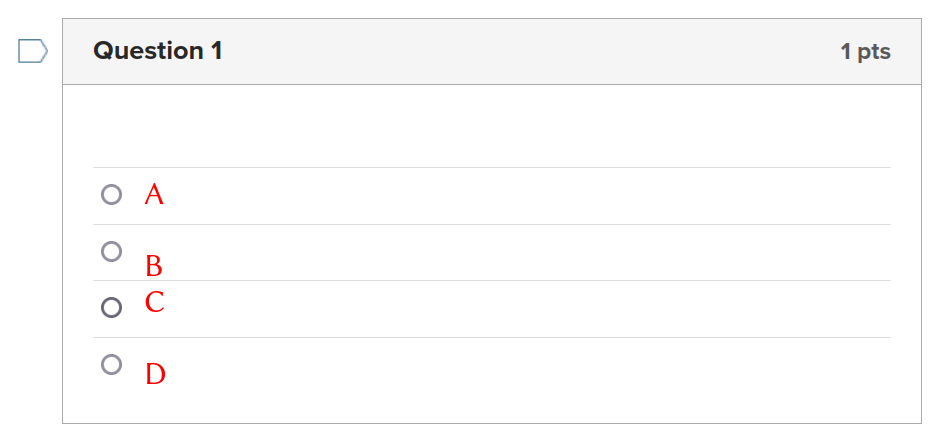
\includegraphics[width=\textwidth]{./figures/Carmen_Q_Example.png}
\end{figure}

\section*{Quizzes, Problem Sets and Examinations Integrity Policies}
\addcontentsline{toc}{section}{Quizzes, Problem Sets and Examinations Integrity Policies}

\textbf{Quizzes and Problem Sets}: Discussions are \textbf{encouraged}, but each person must hand in their own quiz on Carmen.

\textbf{Examinations}: Discussions are \textbf{forbidden}, either face to face or via online discussion board / Social media. You are allowed to refer to course slides, core-econ textbook, lecture videos.

% \subsection*{Extra credits}

% Extra credits: At the end of the semester, I will have you do the Student Evaluation of Instruction (SEI). If I get $80\%$ response rate on SEI by the end of the semester, everyone will get 2 points of extra credits.

\subsection*{Curving}
\addcontentsline{toc}{subsection}{Curving}

If less than $40\%$ of the students get A- or above, I will add some points to everybody until $40\%$ of the students get A- or above, but I don’t expect this to occur.

% \subsection*{Bailout Policy: Midterm \& Final weight change}
% \label{sub:Bailout_Policy__Midterm____Final_weight_change}
% \addcontentsline{toc}{subsection}{Bailout Policy: Midterm \& Final weight change}

% After the midterm exam, there will be a survey on Carmen asking whether you want to change the weight between midterm and final from $ 25 $ points each to $ 10 $ points for midterm and $ 40  $ points for final.
% This survey will due \textbf{before} the final exam date, and you cannot change the weight between midterm and final after you took the final exam.

\subsection*{End-of-semester curtesy grade boost}
\label{sub:End_of_semester_curtesy_grade_boost}
\addcontentsline{toc}{subsection}{End-of-semester curtesy grade boost}

After the final exam and before I submit the grade, there is a grace period where I will accept emails to \textbf{request} the curtesy boost of your semester grade.
Usually, if your semester grade is within $ 1 $ points range of the next letter grade, I will accept the request and boost you to the next letter grade.
For semester grade that has distance larger than $ 1 $ points to the next letter grade, I will access the overall performance to decide whether I will approve the request.

\newpage

% \section*{Course Attendance Policy}

% According to the new ASC policy, \textbf{strictly masking} is required, which means you should wear your mask to cover your mouth and nose.
% Also, the students \textbf{are not allowed to eat or drink} in class.

% The definition of in-person class also redefined by new ASC policy.
% Up to \textbf{24\%} of the class meetings can be online.
% If I cannot teach the course in person due to personal issue, I will make an announcement on \href{https://osu.instructure.com/courses/114824}{Carmen}, and the class will be held online in the \href{https://osu.zoom.us/j/2532324996?pwd=c2cweEphWFMvTVZreHJ0MHNRNUdodz09}{zoom link}.

% The instructor is also required to make reasonable accommodations for students who cannot attend the classes for a period of time, either because of sickness or quarantine.
% My arrangement is to open all my class recordings back in the summer in the \href{https://huijunchen9260.github.io/PrincipleMacroSpring2022.html}{Webpage} so that students who cannot come to class can also reach out the course materials by watching the recorded videos.
% Also, since the office hour is online, those students who cannot attend the in-person meeting can also ask me question on the \href{https://osu.zoom.us/j/2532324996?pwd=c2cweEphWFMvTVZreHJ0MHNRNUdodz09}{zoom link}.


% \newpage

\section*{Tentative Course Schedule}
\addcontentsline{toc}{section}{Tentative Course Schedule}

(Updated: \today)

\newlength\bb
\setlength\bb{\dimexpr .06\textwidth -2\tabcolsep}
\newlength\qq
\setlength\qq{\dimexpr .14\textwidth -2\tabcolsep}
\newlength\rr
\setlength\rr{\dimexpr .3\textwidth -2\tabcolsep}
\newlength\pp
\setlength\pp{\dimexpr .5\textwidth -2\tabcolsep}
\begin{tabular}{|p{\bb}|p{\qq}|p{\rr}|p{\pp}|}
    \hline
        Wk & Days & Quizzes & Topics, Readings and Deadlines for quizzes \\
    \hline
    \hline
        1
        &
        01/08
        \newline
        01/10
        \newline
        01/12
        &
        Syllabus
        &
        Topic: Introducing Syllabus and Class
        \newline
        Reading: Unit 1
        \newline
        Deadline: 01/15 11:59pm
    \\
    \hline
        2
        &
        01/15
        &
        &
        No class: Martin Luther King Day
    \\
    \hline
        2
        &
        01/17
        \newline
        01/19
        &
        &
        Topic: Economic Modelling
        \newline
        Reading: Unit 1 and Unit 2
    \\
    \hline
        3
        &
        01/22
        \newline
        01/24
        \newline
        01/26
        &
        &
        Topic: Consumer
        \newline
        Reading: Unit 3
    \\
    \hline
        4
        &
        01/29
        \newline
        01/31
        \newline
        02/02
        &
        Problem Set 1
        &
        Topic: Firm and Labor
        \newline
        Reading: Unit 6
        \newline
        Deadline: 02/04 11:59pm
    \\
    \hline
        5
        &
        02/05
        \newline
        02/07
        \newline
        02/09
        &
        Problem Set 2
        &
        Topic: Profit Maximization
        \newline
        Reading: Unit 7
        \newline
        Deadline: 02/11 11:59pm
    \\
    \hline
        6
        &
        02/12
        \newline
        02/14
        \newline
        02/16
        &
        Problem Set 3
        &
        Topic: Labor Market
        \newline
        Reading: Unit 9
        \newline
        Deadline: 02/18 11:59pm
    \\
    \hline
        7
        &
        02/19
        \newline
        02/21
        \newline
        02/23
        &
        Problem Set 4
        &
        Topic: Credit Market
        \newline
        Reading: Unit 10
        \newline
        Deadline: 02/25 11:59pm
    \\
    \hline
        8
        &
        02/26
        &
        &
        Midterm Exam
    \\
    \hline
        8
        &
        02/28
        \newline
        03/01
        &
        &
        TBA
    \\
    \hline
\end{tabular}

\begin{tabular}{|p{\bb}|p{\qq}|p{\rr}|p{\pp}|}
    \hline
        Wk & Days & Quizzes & Topics, Readings and Deadlines for quizzes \\
    \hline
    \hline
        9
        &
        03/04
        \newline
        03/06
        \newline
        03/08
        &
        &
        Topic: Fiscal Policy
        \newline
        Reading: Unit 14
    \\
    \hline
        10
        &
        03/11,13,15
        &
        &
        Spring break
    \\
    \hline
        11
        &
        03/18
        \newline
        03/20
        \newline
        03/22
        &
        Problem Set 7
        &
        Topic: Monetary Policy
        \newline
        Reading: Unit 15
        \newline
        Deadline: 03/26 11:59pm
    \\
    \hline
        12
        &
        03/25
        \newline
        03/27
        \newline
        03/29
        &
        Problem Set 8
        &
        Topic: Long-run economic performance
        \newline
        Reading: Unit 16
        \newline
        Deadline: 04/02 11:59pm
    \\
    \hline
        13
        &
        04/01
        \newline
        04/03
        \newline
        04/05
        &
        &
        Topic: Application: The Great Depression
        \newline
        Reading: Unit 17
    \\
    \hline
        14
        &
        04/08
        \newline
        04/10
        \newline
        04/12
        &
        &
        Topic: Application: Asset price bubbles
        \newline
        Reading: Unit 11
    \\
    \hline
        15
        &
        04/17,19,21
        &
        None
        &
        Week for adjustment
    \\
    \hline
        16
        &
        TBA
        &
        None
        &
        Final Exam
    \\
    \hline
\end{tabular}



\newpage

\section*{New General Education Learning Outcomes}
\label{sec:New_General_Education_Learning_Outcomes}
\addcontentsline{toc}{section}{New General Education Learning Outcomes }

Credit: Dr. Darcy Hartman

\textbf{Under the new GE, this course fulfills the GE Foundations requirement for Social and Behavioral Sciences.} 

\textbf{Goals:}
\begin{enumerate}
    \item Successful students will critically analyze and apply theoretical and empirical approaches within the social and behavioral sciences, including modern principles, theories, methods, and modes of inquiry.
    \item Successful students will recognize the implications of social and behavioral scientific findings and their potential impacts.
\end{enumerate}

\textbf{Expected Learning Outcomes:}

Successful students will be able to:

\begin{enumerate}
    \item Explain basic facts, principles, theories, and methods of social and behavioral science.
    \item Explain and evaluate differences, similarities, and disparities among institutions, organizations, cultures, societies, and/or individuals using social and behavioral science.
    \item Analyze how political, economic, individual, or social factors and values impact social structures, policies, and/or decisions.
    \item Evaluate social and ethical implications of social scientific and behavioral research.
    \item Critically evaluate and responsibly use information from the social and behavioral sciences.
\end{enumerate}

Economics 2002.01 will achieve these learning outcomes by teaching students about the theories and methods of social scientific inquiry through discussion of supply and demand at the national level, and the measurement of national income and other macroeconomic measures, along with applications to current events. Students will write a paper on a current event, following the event through the course of the semester. They will perform a critical analysis of the problem and solution utilizing various sources to present their arguments.

Students will learn about the formation and durability of political, economic, and social organizing principles through discussions of the origin and structure of central banks as well as other international organizations, and fiscal and monetary policy. These topics will include discussion of various commonly accepted points of view.

Students will comprehend and assess the nature and values of organizations and polities and their importance in social problem solving and policy making through discussion of fiscal and monetary policy, business cycles and the Federal Reserve Bank, including its values and objectives. In addition, by choosing their own topic, they will have an in-depth look at a current event to study within the context of these principles.

\newpage

\section*{Legacy General Education Course learning outcomes}
\addcontentsline{toc}{section}{Legacy General Education Course learning outcomes}

\textbf{This course fulfills the GE Goals and Expected Learning Outcomes for Social Science: Organizations and Polities.}

\subsection*{Social Science Goal}
\addcontentsline{toc}{subsection}{Social Science Goal}

Students understand the systematic study of human behavior and cognition; the structure of human societies, cultures, and institutions; and the processes by which individuals, groups, and societies interact, communicate, and use human, natural, and economic resources.

\subsection*{Organizations and Polities Expected Learning Outcomes}
\addcontentsline{toc}{subsection}{Organizations and Polities Expected Learning Outcomes}
\begin{enumerate}
    \item Students understand the theories and methods of social scientific inquiry as they apply to the study of organizations and polities.
    \item Students understand the formation and durability of political, economic, and social organizing principles and their differences and similarities across contexts.
    \item Students comprehend and assess the nature and values of organizations and polities and their importance in social problem solving and policy making.
\end{enumerate}

Economics 2002.01 addresses the theories and methods of social scientific inquiry through discussion of supply and demand at the national level, and the measurement of national income and other macroeconomic measures, along with applications to current events.

Students will learn about the formation and durability of political, economic, and social organizing principles through discussions of the origin and structure of central banks as well as other international organizations, and fiscal and monetary policy. These topics will include discussion of various commonly accepted points of view.

Students will comprehend and assess the nature and values of organizations and polities and their importance in social problem solving and policy making through discussion of fiscal and monetary policy, business cycles and the Federal Reserve Bank, including its values and objectives.



\newpage

\section*{Ohio State’s academic integrity policy}
\addcontentsline{toc}{section}{Ohio State’s academic integrity policy}

Academic integrity is essential to maintaining an environment that fosters excellence in teaching, research, and other educational and scholarly activities.
Thus, The Ohio State University and the Committee on Academic Misconduct (COAM) expect that all students have read and understand the University’s Code of Student Conduct, and that all students will complete all academic and scholarly assignments with fairness and honesty.
Students must recognize that failure to follow the rules and guidelines established in the University’s Code of Student Conduct and this syllabus may constitute ``Academic Misconduct.''

The Ohio State University’s Code of Student Conduct (Section 3335-23-04) defines academic misconduct as: ``Any activity that tends to compromise the academic integrity of the University, or subvert the educational process.''
Examples of academic misconduct include (but are not limited to) plagiarism, collusion (unauthorized collaboration), copying the work of another student, and possession of unauthorized materials during an examination.
Ignorance of the University’s Code of Student Conduct is never considered an ``excuse'' for academic misconduct, so I recommend that you review the Code of Student Conduct and, specifically, the sections dealing with academic misconduct.

\textbf{If I suspect that a student has committed academic misconduct in this course, I am obligated by University Rules to report my suspicions to the Committee on Academic Misconduct.} 
If COAM determines that you have violated the University’s Code of Student Conduct (i.e., committed academic misconduct), the sanctions for the misconduct could include a failing grade in this course and suspension or dismissal from the University.

If you have any questions about the above policy or what constitutes academic misconduct in this course, please contact me.

Other sources of information on academic misconduct (integrity) to which you can refer include:
\begin{itemize}
    \item The Committee on Academic Misconduct web pages (COAM Home)
    \item Ten Suggestions for Preserving Academic Integrity (Ten Suggestions)
    \item Eight Cardinal Rules of Academic Integrity (www.northwestern.edu/uacc/8cards.htm)
\end{itemize}

Violating university or course rules as contained in the course syllabus or other information provided to the student in regard to student classroom conduct may result in your being removed from the class rolls.

\subsection*{Other Policies}
\addcontentsline{toc}{section}{Other Policies}

Students with disabilities that have been certified by the Office for Disability Services will be appropriately accommodated.
They should inform the instructor as soon as possible of their needs.
Students who feel that they need an accommodation based on the impact of a disability should contact the Office for Disability Service.
General information is available at http://www.ods.ohio-state.edu.

The core material contained within this syllabus will either be discussed in class or assigned as required reading.

If you decide not to complete the course, please formally withdraw from the class.
Failure to officially withdraw will result in an ``E'' on your transcript and you will have foregone the opportunity to receive a refund (partial or full).

You are expected to be on time to class.
In those events when you do arrive at class late, please find a seat as quietly and unobtrusively as possible.
Do not interrupt class to hand in assignments or request materials.
An opportunity will be provided for these activities at an appropriate time.

We will be doing in-class participation exercises that work via the internet.
Please be sure to bring a mobile device (laptop, tablet, or smartphone) with you to class each day.

\subsection*{Economics Learning Center}
\addcontentsline{toc}{subsection}{Economics Learning Center}

Information can be found at https://economics.osu.edu/economics-learning-center.

\subsection*{Grading scale}
\addcontentsline{toc}{subsection}{Grading scale}
\begin{itemize}
    \item 93–100: A
    \item 90–92.9: A-
    \item 87–89.9: B+
    \item 83–86.9: B
    \item 80–82.9: B-
    \item 77–79.9: C+
    \item 73–76.9: C
    \item 70 –72.9: C-
    \item 67 –69.9: D+
    \item 60 –66.9: D
    \item Below 60: E
\end{itemize}


% \printbibliography

\end{document}

